\chapter{Introduction}
Capturing and understanding of the 3D environment are two fundamental problems for many applications in computer graphics, vision, and robotics community.
%
In the computer, the 3D environment is commonly represented as the textured mesh including geometry and color information. The geometry information is contained in the triangle mesh with a set of vertices and triangles connecting them. Since the color is associated with the surface, it is represented as the surface texture with a UV parameterization and a texture image. First, we associate an additional 2D coordinate with each vertex so that each 3D region is mapped to a 2D parameterization space. The association of the 2D coordinate is called the UV parameterization, and the 2D space is named as the UV space and in the computer graphics community. A texture image is used to store the color in the UV space so that the surface color can be determined by sampling through the mapping. Figure~\ref{fig:intro-texture-represent} illustrates how the textured mesh is represented in the computer.
\begin{figure}
    \centering
    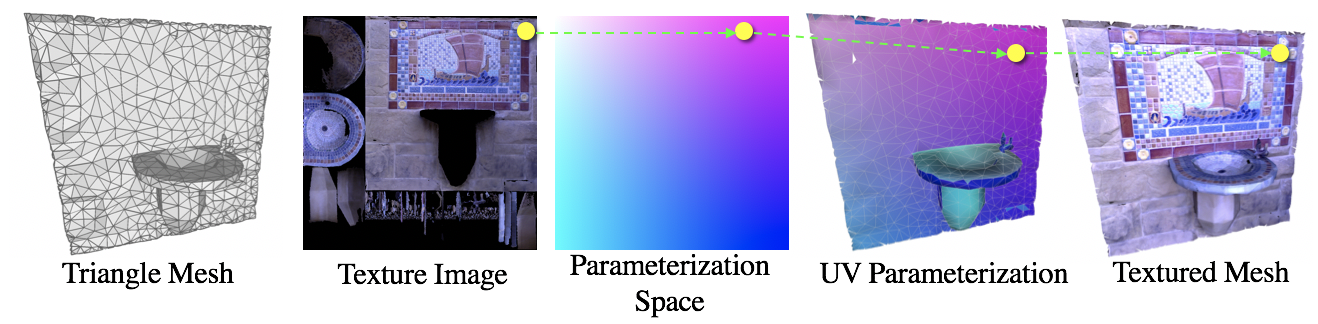
\includegraphics[width=\linewidth]{intro/texture-represent.png}
    \caption{Textured mesh representation in the computer. The geometry information is stored as a triangle mesh. The color information is stored as a surface texture with a UV parameterization for all vertices and a texture image stored in the parameterization space.}
    \label{fig:intro-texture-represent}
\end{figure}
We focus on the surface texture processing -- reconstructing and understanding the surface texture based on commodity RGB-D cameras.

By reconstruction, we aim at producing high-quality texture from inaccurate and low-quality scanning data. The wide availability of consumer range cameras has spurred extensive research in geometric reconstruction of real-world objects and scenes, with state-of-the-art 3D reconstruction approaches now providing robust camera tracking and 3D surface reconstruction~\cite{newcombe2011kinectfusion,izadi2011kinectfusion,whelan2015elasticfusion,dai2017bundlefusion}. However, producing a photorealistic textured mesh of real-world environments requires not only geometric reconstruction but also high-quality color reconstruction.
Unfortunately, due to noisy input data, poorly estimated surface geometry, misaligned camera parameters, unmodeled optical distortions, and view-dependent lighting effects,  aggregating multiple real-world images into high-quality, realistic surface textures is still a challenging problem. We aim at addressing this problem by minimizing color inconsistency or jointly optimizing the texture with a learned metric, as described in section~\ref{intro:texture-recon}.

While our deep metric can be implemented with an image convolutional neural network (CNN) as a widely-studied deep learning technique, one followup in this thesis is to directly apply a CNN in the texture domain of the 3D surface.
%
The advantage of applying CNN operator on 3D data over 2D images is obvious: convolutions directly operated in 3D data are relatively unaffected by view-dependent image effects, such as perspective, occlusion, lighting, and background clutter.
%
There has been a lot of recent works on the semantic segmentation of 3D data using 3D CNN. However, the resolution of current 3D representations is generally quite low (2cm is typical), and so the ability of 3D CNNs to discriminate fine-scale semantic patterns is usually far below their color image counterparts \cite{long2015fully,he2017mask}.
%
We believe a 2D CNN applied in the texture domain of the 3D surface can address the above issue, and the key challenge is to obtain a consistent and canonical surface parameterization that maps the 3D surface into a 2D space where 2D convolutions can apply.
%
We find that this challenge is related to the seamless surface parameterization problem in the computational geometry community. While this problem has been studied for more than a decade, the existing state-of-the-art method formulated as a mixed-integer programming problem (NP-hard), where an effective and robust solution is unavailable.
%
We reformulate the problem and obtain a robust and efficient seamless parameterization for the geometry of a complex 3D environment (section~\ref{intro:param}).


With the surface parameterization, we propose a surface convolution operator that extracts effective features in the parameterization space (section~\ref{intro:texture-learn}).
%
Specifically, we apply our convolution operator in our well-defined geodesic neighborhood where each point is locally parameterized with a 2D coordinate based on our seamless parameterization.
%
We make our novel convolution operator four-way rotationally symmetric to canonicalize the feature extraction with the existence of orientation singularities in the parameterization.
%
Our surface convolution is a 2D operator that effectively handles, and thereby outperforming other less efficient dense 3D convolution operators.
%
We find that the surface parameterization serves as not only a basis for surface convolution operators to apply but also useful information that is highly-correlated and learnable from the color signals. Therefore, we create a dataset with pairs of RGB images and pre-computed 3D canonical frames from the scanning data and train a neural network to predict frames from color signals. Our network enables various applications including surface normal estimation, feature matching and augmented reality (section~\ref{intro:frame}).

In summary, this thesis addresses the surface texture processing problem from the perspective of texture reconstruction (section~\ref{intro:texture-recon}) and texture understanding. We further identify the texture understanding problem as the surface parameterization problem (section~\ref{intro:param}) and learning methods based on it (section~\ref{intro:understand}). We summarize the contribution of the thesis in section~\ref{intro:contribution}.

\section{Texture Reconstruction}
\label{intro:texture-recon}
This section discusses our motivation and approaches for texture reconstruction. We discuss the related works about texture reconstruction is section~\ref{related:texture-recon} and introduce the technical details of our approaches including \textit{3DLite}~\cite{huang20173dlite} and \textit{Adversarial Texture Optimization}~\cite{huang2020adversarial} in chapter~\ref{chapter:texture-recon}.

\paragraph*{Motivation} RGB-D scanning has made rapid advances in recent years with the introduction of commodity range sensors, such as the Microsoft Kinect, Intel RealSense, or Google Tango. In this scenario, the textured mesh can be produced by fusing depth images into the geometry and color images into the surface texture.
State-of-the-art online and offline 3D geometry reconstruction methods now allow remarkable capture and digitization of a variety of real-world environments, with faithful geometric fidelity~ \cite{newcombe2011kinectfusion,izadi2011kinectfusion,chen2013scalable,niessner2013real,choi2015robust,dai2016bundlefusion}.
Although the intended applications of these methods cover a variety of gaming, virtual reality, and augmented reality scenarios, the quality of the resulting 3D models remains far from the caliber of artist-modeled content.
In particular, current reconstructions still suffer from noise, oversmoothing, and holes, rendering them inadequate for use in production applications. Therefore, both the geometry and the texture from the 3D reconstruction are problematic for the real applications.

\begin{figure}
    \centering
    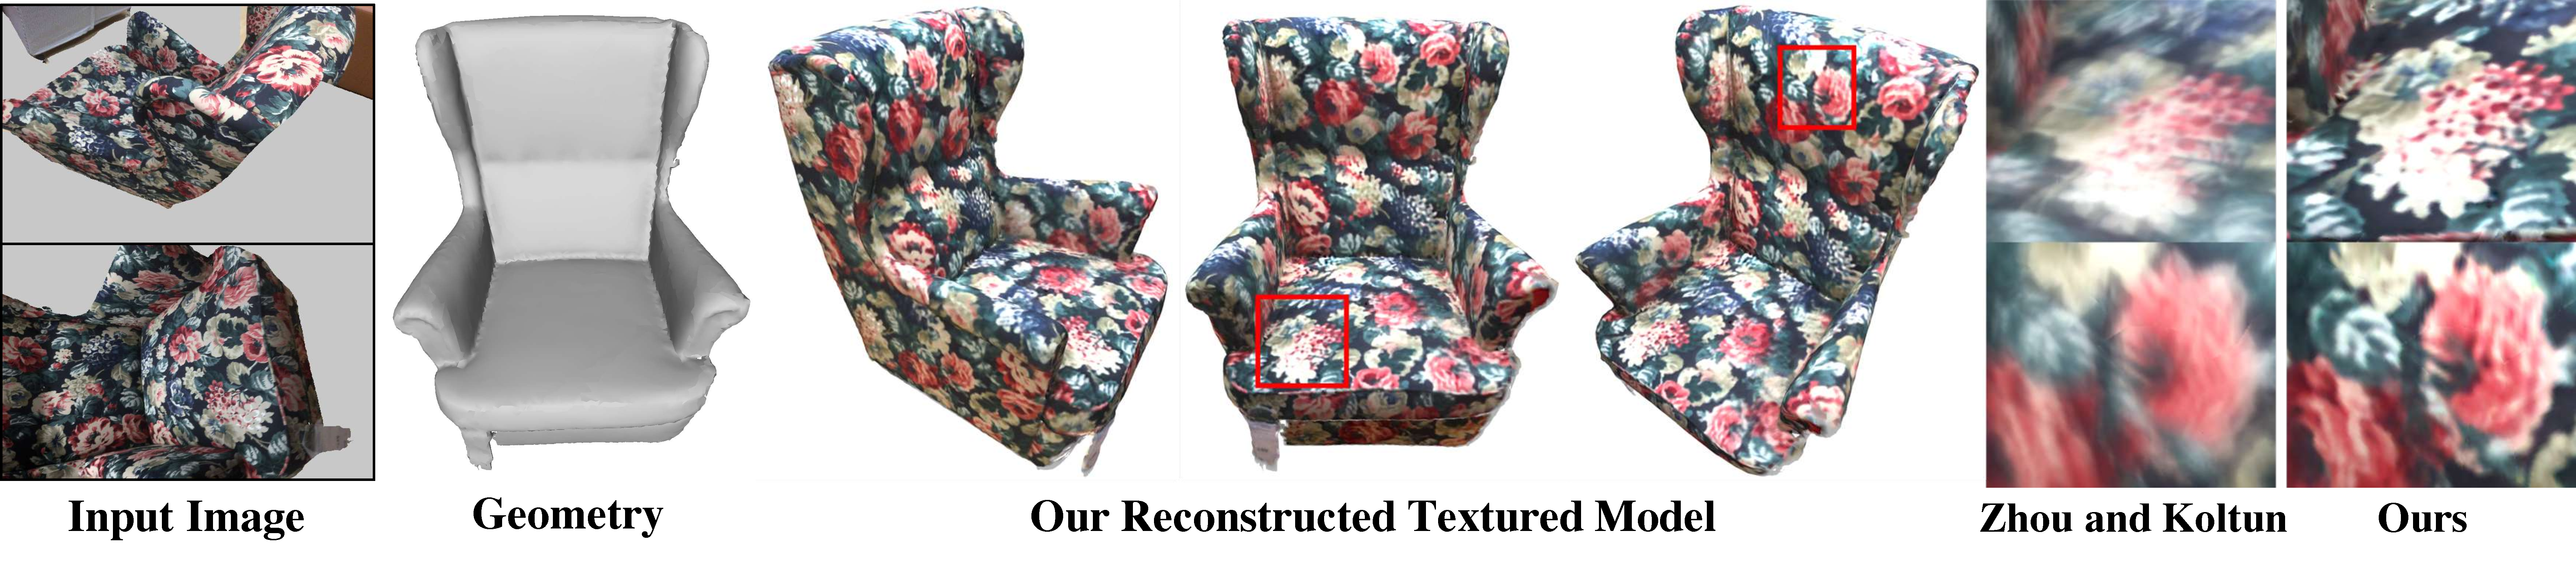
\includegraphics[width=\textwidth]{texturegen/figures/teaser-n.pdf}
    \caption{Our goal is to reconstruct high-quality textures from the 3D scan with aligned input images. Traditional methods optimize for a parametric color map to reduce misalignment error (Zhou and Koltun~\cite{zhou2014color}). We seek better color consistency optimization and view aggregation method, and further derive a flexible texture optimization framework based on a learned metric that is robust to common scanning errors.}
    \label{fig:toptim-teaser}
\end{figure}
From the graphics perspective, we observe that the surface textures are more important to visual perception than geometry; for instance, many video games make use of techniques such as billboarding or bump mapping~\cite{decoret1999multi}
to achieve high-detail visuals at low cost, with an almost imperceptible difference to using accurate geometry. Therefore, accurate geometric reconstruction is heavy and unnecessary, while light-weighted approximations of the scanning geometry with artifact-free primitives or CAD models are favored for interactive applications including gaming and virtual/augmented reality. 
Thus, our works assume inaccurate geometries from reconstructed from the scan or even further approximated with light-weight primitives and CAD models and focus on the high-quality texture mapping given the input as the RGB images and misaligned geometry as shown in figure~\ref{fig:toptim-teaser}.

High-quality texture reconstruction is a challenging problem. The color quality of existing 3D reconstruction methods often suffers from artifacts due to motion blur and rolling shutter from commodity color cameras. 
This is compounded by oversmoothing and camera pose micro-misalignments due to popular reconstruction techniques.
For instance, the seminal volumetric fusion work~\cite{curless1996volumetric} is commonly used to generate a 3D model from input RGB-D frames by performing a weighted average over projected depth and color observations.
While effectively regularizing out noise, this also results in oversmoothed geometry and color.
Additionally, since camera poses are computed from imperfect color and noisy, relatively low-quality depth, they often suffer from micro-drift, which further exacerbates resulting visual artifacts such as ghosting and oversmoothing. To overcome these problems, various approaches have been developed to optimize color textures using models to adjust camera poses~\cite{zhou2014color}, distort images~\cite{bi2017patch,zhou2014color}, and balance colors \cite{zhou2014color}.  However, these prior approaches are not expressive enough and/or their optimization algorithms are not robust enough to handle the complex distortions and misalignments commonly found in scans with commodity cameras -- and therefore they fail to produce high-quality results for typical scans as shown in the results from Zhou and Koltun~\cite{zhou2014color} in Figure~\ref{fig:toptim-teaser}.

To address these issues, we propose two approaches from different perspectives. The first approach~\cite{huang20173dlite} seeks better color consistency optimization and view aggregation by optimizing an explicit parametric models. The second approach~\cite{huang2020adversarial} further derives a flexible texture optimization framework based on a learned metric that is robust to common scanning errors (right side of Figure~\ref{fig:toptim-teaser}).
 
\paragraph*{Geometry Priors}
Our first approach, \emph{3DLite}~\cite{huang20173dlite}, generates lightweight, complete, CAD-like models of large-scale indoor scenes before we reconstruct high-quality textures.
%
We take as input an RGB-D video sequence from a handheld commodity sensor and first reconstruct the scene with existing 3D reconstruction methods.
Since we aim to generate complete scenes and sharp, clean textures, we employ a primitive-based abstraction to represent the scanned environments.
In particular, we use plane primitives, as planes facilitate texture mapping as well as scene completion through extrapolation, thus generating a denoised geometric representation of the scene.
%
We first optimize for these primitives under a Manhattan assumption, since man-made environments are often designed in such highly structured fashion.
To complete the scene geometry in occluded regions, we formulate a new hole-filling approach by extrapolating the planar primitives according to unknown space as seen by the camera trajectory.
That is, we respect the known empty space in the scene and only fill holes in regions unseen by the camera.
This generates a complete geometric representation of the scene.
%
Our second approach, \emph{Adversarial Texture Optimization}~\cite{huang2020adversarial}, learns a deep-metric that tolerates complex misalignment between image observations and the target geometry. Therefore, we can replace the scanning geometry with clean human-created CAD models with geometry misalignments but still perform decent texture optimization.

\paragraph*{Parametric Texture Optimization}
Our first approach~\cite{huang20173dlite} performs a novel texture optimization to map the scene geometry with sharp colors from the input RGB data.
Since camera poses estimated from noisy RGB-D data are prone to micro-drift, our texture optimization step solves for refined rigid and non-rigid image alignments, optimizing for photo-consistency using both sparse color and dense geometric information.
%
Zhou \textit{et al.}~\cite{zhou2014color} optimize purely for a dense energy term remains sensitive to initial poses and easy to end up in local minima. Therefore, we build upon them and employ a sparse-to-dense optimization, using sparse color features and geometric primitive constraints to help reach the basin of convergence of the dense photo-consistency energy.
%
To mitigate the effects of motion blur and auto-exposure, we perform an exposure correction and select and stitch together only the sharpest regions of the input RGB images, obtaining globally consistent, sharp colors. While existing methods reduce blurriness artifacts caused by average aggregation with single view selection~\cite{dessein2014seamless}, we further take pixel sharpness into consideration in the existence of motion blur. We select the best view for each region to balance the visual sharpness and color consistency of boundaries between neighboring regions with different views selected, which is modeled as a multi-label graph-cut problem~\cite{boykov2001fast}.

\paragraph*{Adversarial Metric for Texture Optimization}
Prior approaches depend on explicit models and color consistency optimization, and are not expressive enough and/or their optimization algorithms are not robust enough to handle the complex distortions and misalignments commonly found in scans with commodity cameras.

\begin{figure}
    \centering
    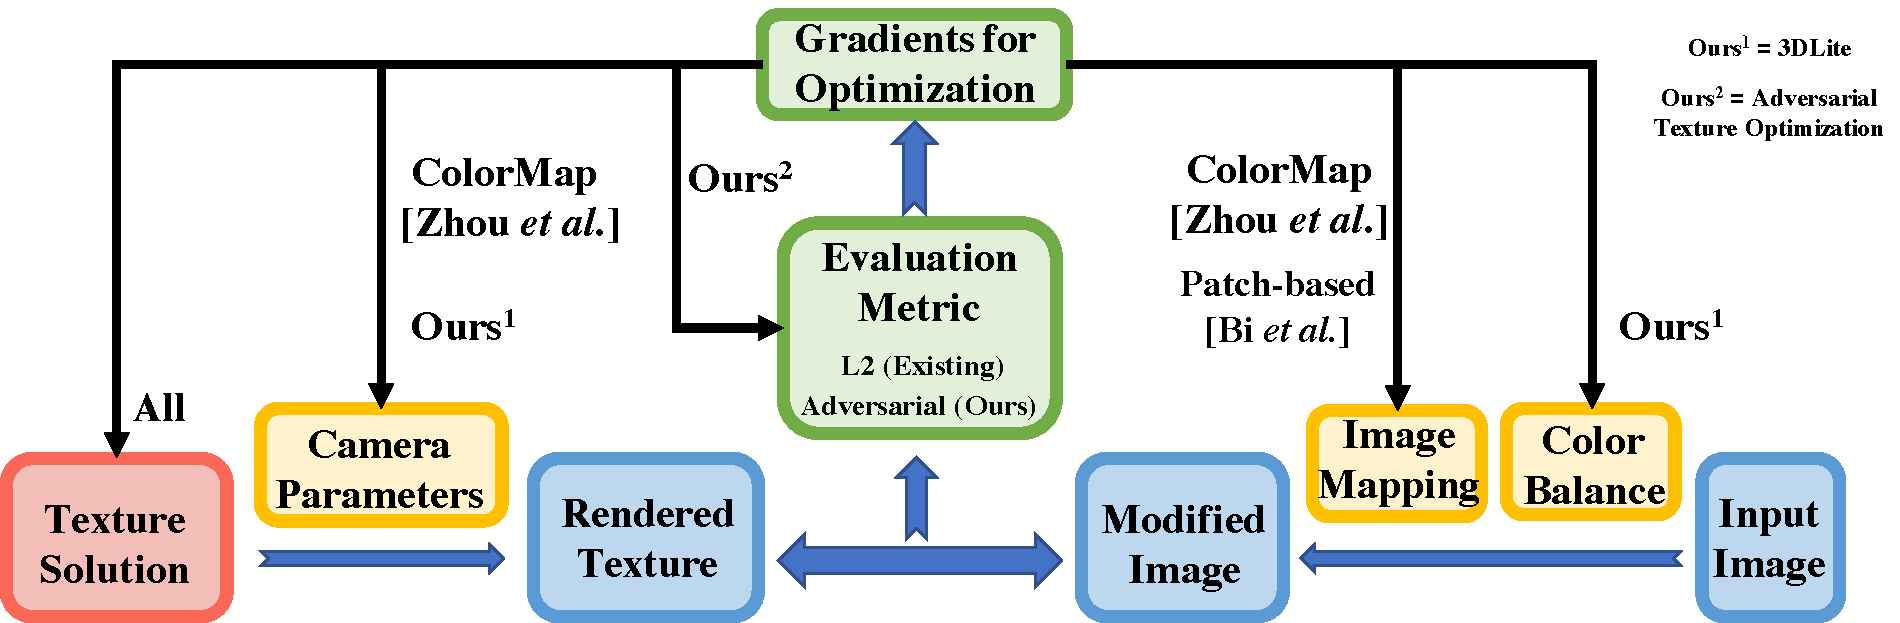
\includegraphics[width=\linewidth]{texturegen/figures/concept.pdf}
    \caption{All methods target at optimizing a texture solution. Existing methods optimize the texture jointly with camera parameters~\cite{zhou2014color,huang20173dlite}, image mapping~\cite{zhou2014color,bi2017patch} or color balance~\cite{huang20173dlite}. Instead, we jointly solve texture with an adversarial evaluation metric to tolerate the errors.}
    \label{fig:toptim-concept}
\end{figure}
To address these issues, our second approach~\cite{huang2020adversarial} proposes a flexible texture optimization framework based on a learned metric that is robust to common scanning errors.
% the scanning errors tuned separately for each individual scan. 
 The key idea behind our approach is to account for misalignments in a {\em learned objective function} of the texture optimization.   
 Rather that using a traditional object function, like $L1$ or $L2$, we learn a new objective function (adversarial loss) that is robust to the types of misalignment present in the input data.  This novel approach eliminates the need for hand-crafted parametric models for fixing the camera parameters \cite{zhou2014color,huang20173dlite} or image mapping \cite{bi2017patch,zhou2014color} or color balance \cite{huang20173dlite} (bottom row of Figure~\ref{fig:toptim-concept}) and replaces them all with a learned evaluation metric (green box in Figure~\ref{fig:toptim-concept}).   As such, it adapts to the input data.
 
Inspired by the success of adversarial networks in image synthesis~\cite{goodfellow2014generative}, we propose to use a learned conditional discriminator to serve our {\em objective function} and jointly optimize the color texture of a reconstructed surface with this discriminator.
The condition is a captured image $I_A$ from the source view $V_A$, and the query is either (i) ``real:'' a second captured image $I_B$ (from an auxiliary view $V_B$) projected onto the surface and then rendered back to $V_A$, or (ii) ``fake:'' an image of the optimized synthetic texture rendered to view $V_A$. By optimizing the surface texture while jointly training this conditional discriminator, we aim to produce a texture that is indistinguishable from reprojections of captured images from all other views.  
%
During the optimization, the discriminator learns invariance to the misalignments and distortions present in the input dataset, while recognizing synthetic artifacts that do not appear in the real images, like local blurs and seams.  The synthesized textures optimized to fool the discriminator appear more realistic than in previous approaches.

Our experiments show that our adversarial optimization framework produces notably improved performance compared to state-of-the-art methods, both quantitatively on synthetic data and qualitatively on real data. 
Moreover, since it tolerates gross misalignments, we are able to generate realistic textures on CAD models which have been only roughly aligned to 3D scans, in spite of large mismatches in surface geometry. 
This opens up the potential to produce CAD models with realistic textures for content creation.

\section{Surface Parameterization}
\label{intro:param}
While our adversarial texture optimization~\cite{huang2020adversarial} uses image convolution, it is more straightforward to perform convolution directly in the parameterized texture space for texture understanding. This section discusses the seamless surface parameterization as the necessary step towards texture understanding, and formulate it as a quadrangulation problem. We discuss the related works in section~\ref{related:param} and the technical details for our quadrangulation method in chapter~\ref{chapter:param}.

\paragraph*{Motivation} For adversarial texture optimization~\cite{huang2020adversarial}, we apply the 2D convolution to learn a misalignment-tolerant metric in the image space. A natural followup is to extract the features for the surface texture by directly applying the 2D convolution in the texture domain. While convolutions directly operated in 3D data are relatively unaffected by view-dependent image effects compared to image-based convolutions, the resolution of current 3D representations is generally quite low given higher dimensions of the data. Fortunately, texture signals lie on the surface instead of the whole 3D volume. It opens the opportunity for us to parameterize the surface using a 2D domain and apply a 2D convolution in the parameterization space. We observe the key difference between 2D images and 3D surfaces is that the image coordinate system serves as a consistent global definition of how the 2D domain is parameterized, while there is no global consistent definition of surface parameterization in 3D.

 \begin{figure}
  \centering
  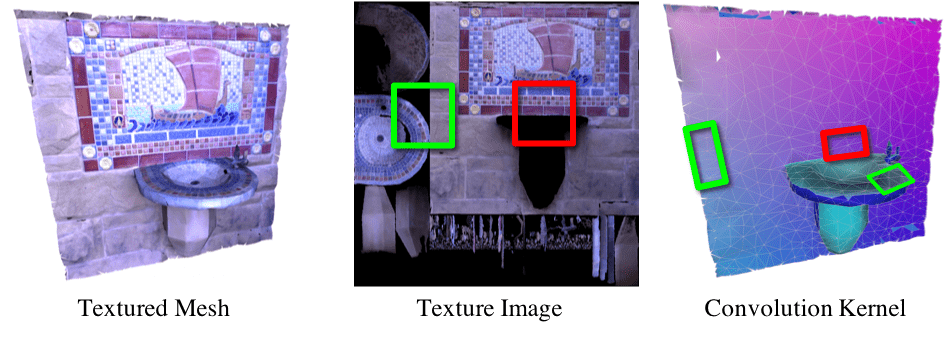
\includegraphics[width=0.8\linewidth]{intro/uvconv.png}
  \caption{Limitation of convolutions with a general UV parameterization. The convolution applied to the texture image incorrectly aggregates disconnected regions (green) and incorporates unexpected boundaries (red).}
  \label{fig:intro-uv-param}
\end{figure}
For example, the most straightforward idea is to directly use general UV parameterization. However, convolution applied to the texture image suffers can cause problems by breaking the connectivity information in the 3D. As shown in figure~\ref{fig:intro-uv-param}, the green convolution kernel incorrectly aggregates disconnected regions of the mesh. Additionally, the red convolution kernel in the texture image reaches the boundaries, while ideally, this should not happen since the center is far from the surface boundary.
 \begin{figure}
    \centering
     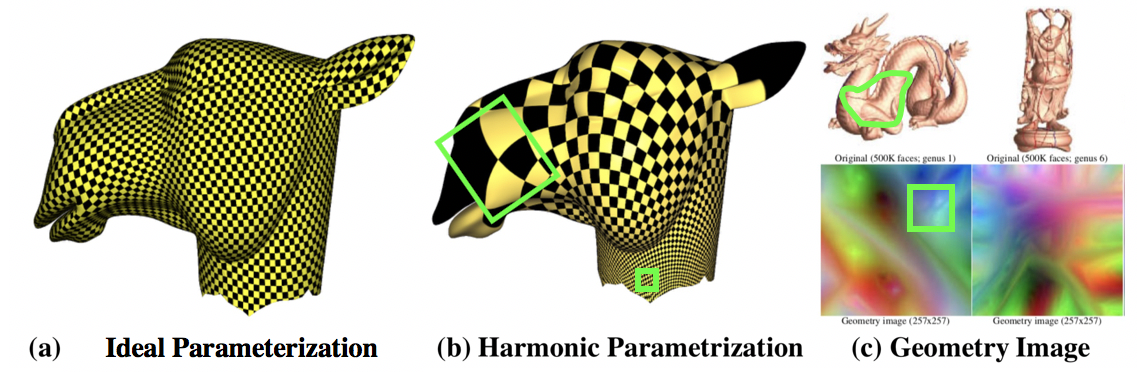
\includegraphics[width=0.8\linewidth]{quadriflow/param.png}
     \caption{(a) With an ideal parameterization, we can get the surface parameterization aligned with shape features with negligible distortion. (b) Harmonic parameterization leads to high distortion in the scale. (c) Geometry images~\cite{gu2002geometry} result in high distortion in the orientation.}
     \label{fig:intro-quadriflow-param}
 \end{figure}
Other well-known parameterization methods can also cause different problems. In figure~\ref{fig:intro-quadriflow-param}, the receptive field of the convolution (marked as green edges) can have significant different scales with harmonic parameterization or irregular neighborhoods with geometry images~\cite{gu2002geometry}. We argue that an ideal parameterization for convolution should be regular, uniform and seamlessly connected. In this case, the receptive field is regular and canonicalized with the same shape and size. Such a parameterization is shown in figure~\ref{fig:intro-quadriflow-param}(a), where the surface is seamlessly parameterized and visually looks like a uniform-scale quadrilateral mesh. Therefore, to tackle the texture convolution problem, we first build a robust and scalable quadrangulation algorithm to convert a general triangle mesh as a quadrilateral mesh as \textit{Quadriflow}~\cite{huang2018quadriflow}.

\paragraph*{Orientation and Singularity} State-of-the-art algorithms for quadrilateral surface meshing typically compute, as a first step, an \emph{orientation field} that assigns local coordinate axes to some points on the input surface \cite{knupp1995mesh,ray2006periodic,kalberer2007quadcover,bommes2009mixed}. The {\em Instant Field-Aligned Meshes} \mbox{algorithm} of Jakob et al.~\cite{jakob2015instant} subsequently computes a \emph{position field} that assigns local coordinates %(in the frame of the local coordinate axes)%
to those points. The orientation field determines the directions of the edges of a quadrilateral mesh, and the position field determines where the mesh vertices are placed. Ideally, both fields should vary smoothly over the surface, while obeying constraints that help to align the mesh with the sharp edges and the curvature of the object.

Both types of fields can have irregularities called \emph{singularities}. If the fields are defined continuously over the surface, a singularity is a region where one of the fields is not locally smooth.
The pitfall of these singularities is that the quad mesh subsequently produced is likely to have an \emph{irregular vertex}---a vertex whose valence is not 4---near the singularity. 
Unfortunately, irregular vertices can cause problems for applications; for instance, they cause unsightly visual artifacts in Catmull--Clark subdivision, or additional work for an artist to edit a model. In our texture understanding scenario, such irregularity means that our convolution kernels are highly distorted or not canonically oriented near the singularity positions.

Algorithms that rely purely on local mesh computations are fast, but they produce meshes with many singularities. It is possible to modify the fields to move singularities and sometimes even to eliminate them; but eliminating a singularity
usually involves merging pairs of singularities located all around the geometry, which is ``nonlocal.'' 
A global view of quad meshing taken by Bommes et al.~\cite{bommes2009mixed}, who cast the problem of seamless global parametrization as a mixed-integer constrained optimization problem (MIP).
The method produces quadrilateral surface meshes of very high quality, but it is slow and it does not scale well to large meshes. By contrast, the much more efficient Instant Meshes algorithm of Jakob et al.~\cite{jakob2015instant} uses local smoothing operators to compute an orientation field and a position field quickly. Their method is scalable and produces high-quality quad-dominant meshes without much distortion. However, it may produce singularities in the position field in addition to singularities in the orientation field.

\paragraph*{Our Formulation} We present \emph{QuadriFlow}~\cite{huang2018quadriflow}, a scalable, robust algorithm for automatic quad meshing that builds upon Instant Meshes but uses a global method to remove all the singularities from the position field.
We do not change the orientation field, which typically has many fewer singularities. Our method solves a minimum cost network flow problem as a subproblem, for which efficient algorithms are available. The speed and reliability of our algorithm can enable designers to work on a modeling task interactively and extract a quad mesh in less than a second for tens of thousands of faces, and enable physical simulations to perform per-timestep remeshing updates. Our current implementation is a \emph{remeshing} algorithm, meaning that its input is a triangular mesh of the input surface (like many other quad meshing algorithms), though it could be modified to take a point cloud input as Instant Meshing does.

We view singularity-free position field computation as a globally constrained optimization problem.
Unlike Bommes et al., we do not solve the problem by mixed-integer programming. Instead, we split it into three stages.
\begin{itemize}
\item Compute the orientation and position fields just as Jakob et al.\ do, without enforcing additional constraints.
\item Enforce our constraints by modifying only the integer variables of the position field, changing the integers as little as possible.
\item Re-optimize the continuous variables of the position field with the integer variables held fixed.
\end{itemize}
The third stage is not difficult, requiring the solution of a linear system. Our main contribution is a fast and effective method for the second, largely combinatorial stage. Because of the regularity constraints, the second stage is a mixed-integer programming problem, for which it is NP-hard to find an optimal solution, but we can obtain good approximate solutions in practice. We reduce the problem to an integer linear program (ILP). We approximate the ILP as an easier \emph{minimum cost network flow} (MCF) problem, which can be solved in polynomial time~\cite{klein1967primal}. We further improve efficiency by a multi-resolution algorithm. To enforce consistent triangle orientations (no inverted triangles), we impose a set of quadratic inequality constraints. We are able to satisfy most of these constraints through simple greedy edge contractions; we find we can satisfy most of the remaining difficult ones by locally solving a small boolean satisfiability problem (SAT).

By replacing the MIP solver with an MCF solver that globally reduces the number of singularities, plus edge contractions and an SAT solver that locally impose triangle orientation constraints, we obtain a scalable quad remesher that produces many fewer singularities than Instant Meshes, often by a factor of four, while being much faster than the method of Bommes et al. QuadriFlow remeshes a one-million triangle mesh in 5 seconds, which is comparable to the interactive method of Ebke et al.~\cite{ebke2016interactively}. Our meshes have less distortion compared to other global methods, and rarely suffer from nonmanifold structure or holes, thanks to the consistent orientation constraints. In a test on 17,000$+$ surfaces created from ShapeNet~\cite{chang2015shapenet}, QuadriFlow robustly removed all the singularities from every discrete position field.
 
\section{Texture Understanding}
\label{intro:understand}
With the powerful seamless parameterization of the surface, we are able to explore the texture understanding problem. This thesis explores the semantic understanding problem with the parameterized textures as well as the 3D frame understanding given the RGB images.

\subsection{Semantics from Texture}
\begin{figure}
    \begin{center}
        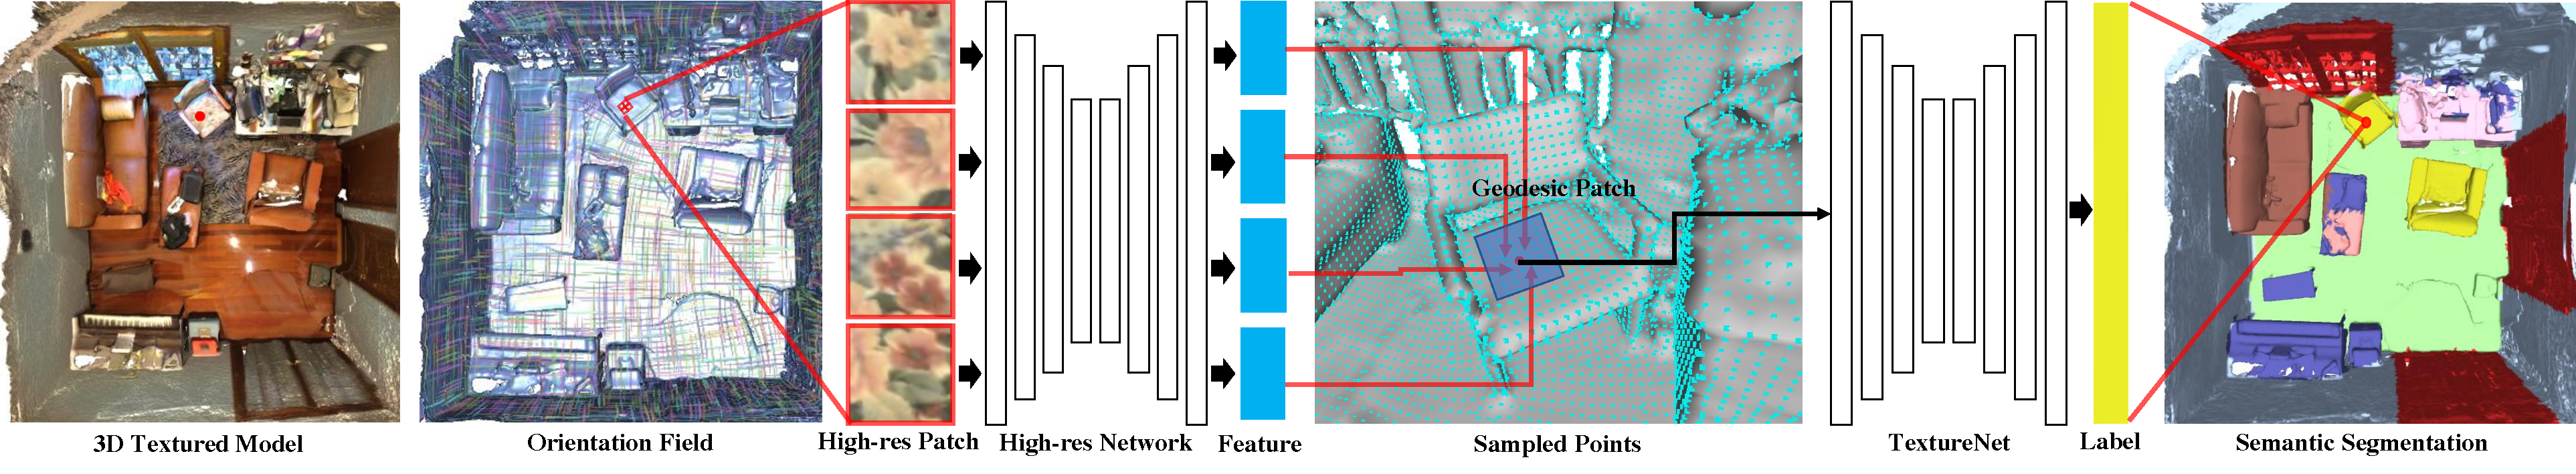
\includegraphics[width=\linewidth]{texturenet/teaser/teaser.pdf}
        \caption{TextureNet takes as input a 3D textured mesh.  The mesh is parameterized with a consistent 4-way rotationally symmetric (4-RoSy) field, which is used to extract oriented patches from the texture at a set of sample points.   Networks of 4-RoSy convolutional operators extract features from the patches and used for 3D semantic segmentation.}
        \label{fig:texturenet-teaser}
    \end{center}    
\end{figure}
\label{intro:texture-learn}
Given the robust seamless surface parameterization, we are able to explore the semantic understanding from the texture signals. We design TextureNet~\cite{huang2018texturenet} as a neural network architecture (figure~\ref{fig:texturenet-teaser}) to extract features from high-resolution signals associated with the 3D surface meshes (e.g., color texture maps).
There has been a lot of recent work on the semantic segmentation of 3D data using convolutional neural networks (CNNs).  Typically, features extracted from the scanned inputs (e.g., positions, normals, height above ground, colors, etc.) are projected onto a coarse sampling of 3D locations, and then a network of 3D convolutional filters is trained to extract features for semantic classification -- e.g., using convolutions over voxels \cite{wu20153d,maturana2015voxnet,qi2016volumetric,song2017semantic,dai2017scannet,dai2018scancomplete}, octrees \cite{riegler2017octnet}, point clouds \cite{qi2017pointnet,qi2017pointnet++}, or mesh vertices \cite{masci2015geodesic}.  The advantage of these approaches over 2D image-based methods is that convolutions operate directly on 3D data, and thus are relatively unaffected by view-dependent image effects, such as perspective, occlusion, lighting, and background clutter.   However, the resolution of current 3D representations is generally quite low (2cm is typical), and so the ability of 3D CNNs to discriminate fine-scale semantic patterns is usually far below their color image counterparts \cite{long2015fully,he2017mask}.

To address this issue, we propose a new convolutional neural network, \emph{TextureNet}~\cite{huang2018texturenet}, with a 2D convolution kernel that extracts features directly from high-resolution signals associated with 3D surface meshes.  Given a map that associates high-resolution signals with a 3D mesh surface (e.g., RGB photographic texture), we define convolutional filters that operate on those signals within domains defined by geodesic surface neighborhoods.   This approach combines the advantages of feature extraction from high-resolution signals (as in \cite{dai20183dmv}) with the advantages of view-independent convolution on 3D surface domains (as in \cite{tatarchenko2018tangent}).

During our investigation of this approach, we had to address several research issues, the most significant of which is how to define geodesic neighborhoods of a mesh.   One approach could be to compute a global UV parameterization for the entire surface and then define convolutional operators directly in UV space; however, that approach may induce significant deformations due to flattening, not always follow surface features, and/or produce seams at surface cuts.  Another approach could be to compute UV parameterizations for local neighborhoods independently; however, then adjacent neighborhoods might not be oriented consistently, reducing the ability of a network to properly learn orientation-dependent features.   Instead, we compute a 4-RoSy (four-fold rotationally symmetric) field on the surface using QuadriFlow~\cite{huang2018quadriflow} and define a new 4-RoSy convolutional operator that explicitly accounts for the 4-fold rotational ambiguity of the cross-field parameterization. A 4-RoSy (four-way rotationally symmetric) field is a configuration of 4 orthogonal tangent directions associated with each vertex in the shape of a cross that varies smoothly over the mesh surface.  Since the 4-RoSy field from QuadriFlow has no seams, aligns to shape features, induces relatively little distortion, has few singularities, and consistently orients adjacent neighborhoods (up to 4-way rotations), it provides an attractive trade-off between distortion and orientation invariance.

Results on 3D semantic segmentation benchmarks show an improvement of the 4-RoSy convolution on surfaces over alternative geometry-only approaches (by 6.4\%), plus significantly further improvement when applied to high-resolution color signals (by 6.9-8.2\% ).  With ablation studies, we verify the importance of the consistent orientation of a 4-RoSy field and demonstrate that our sampling and convolution operator works better than other alternatives.

\subsection{FrameNet: Canonical Frame Understanding from RGB Images}
\label{intro:frame}
 \begin{figure}
    \centering
    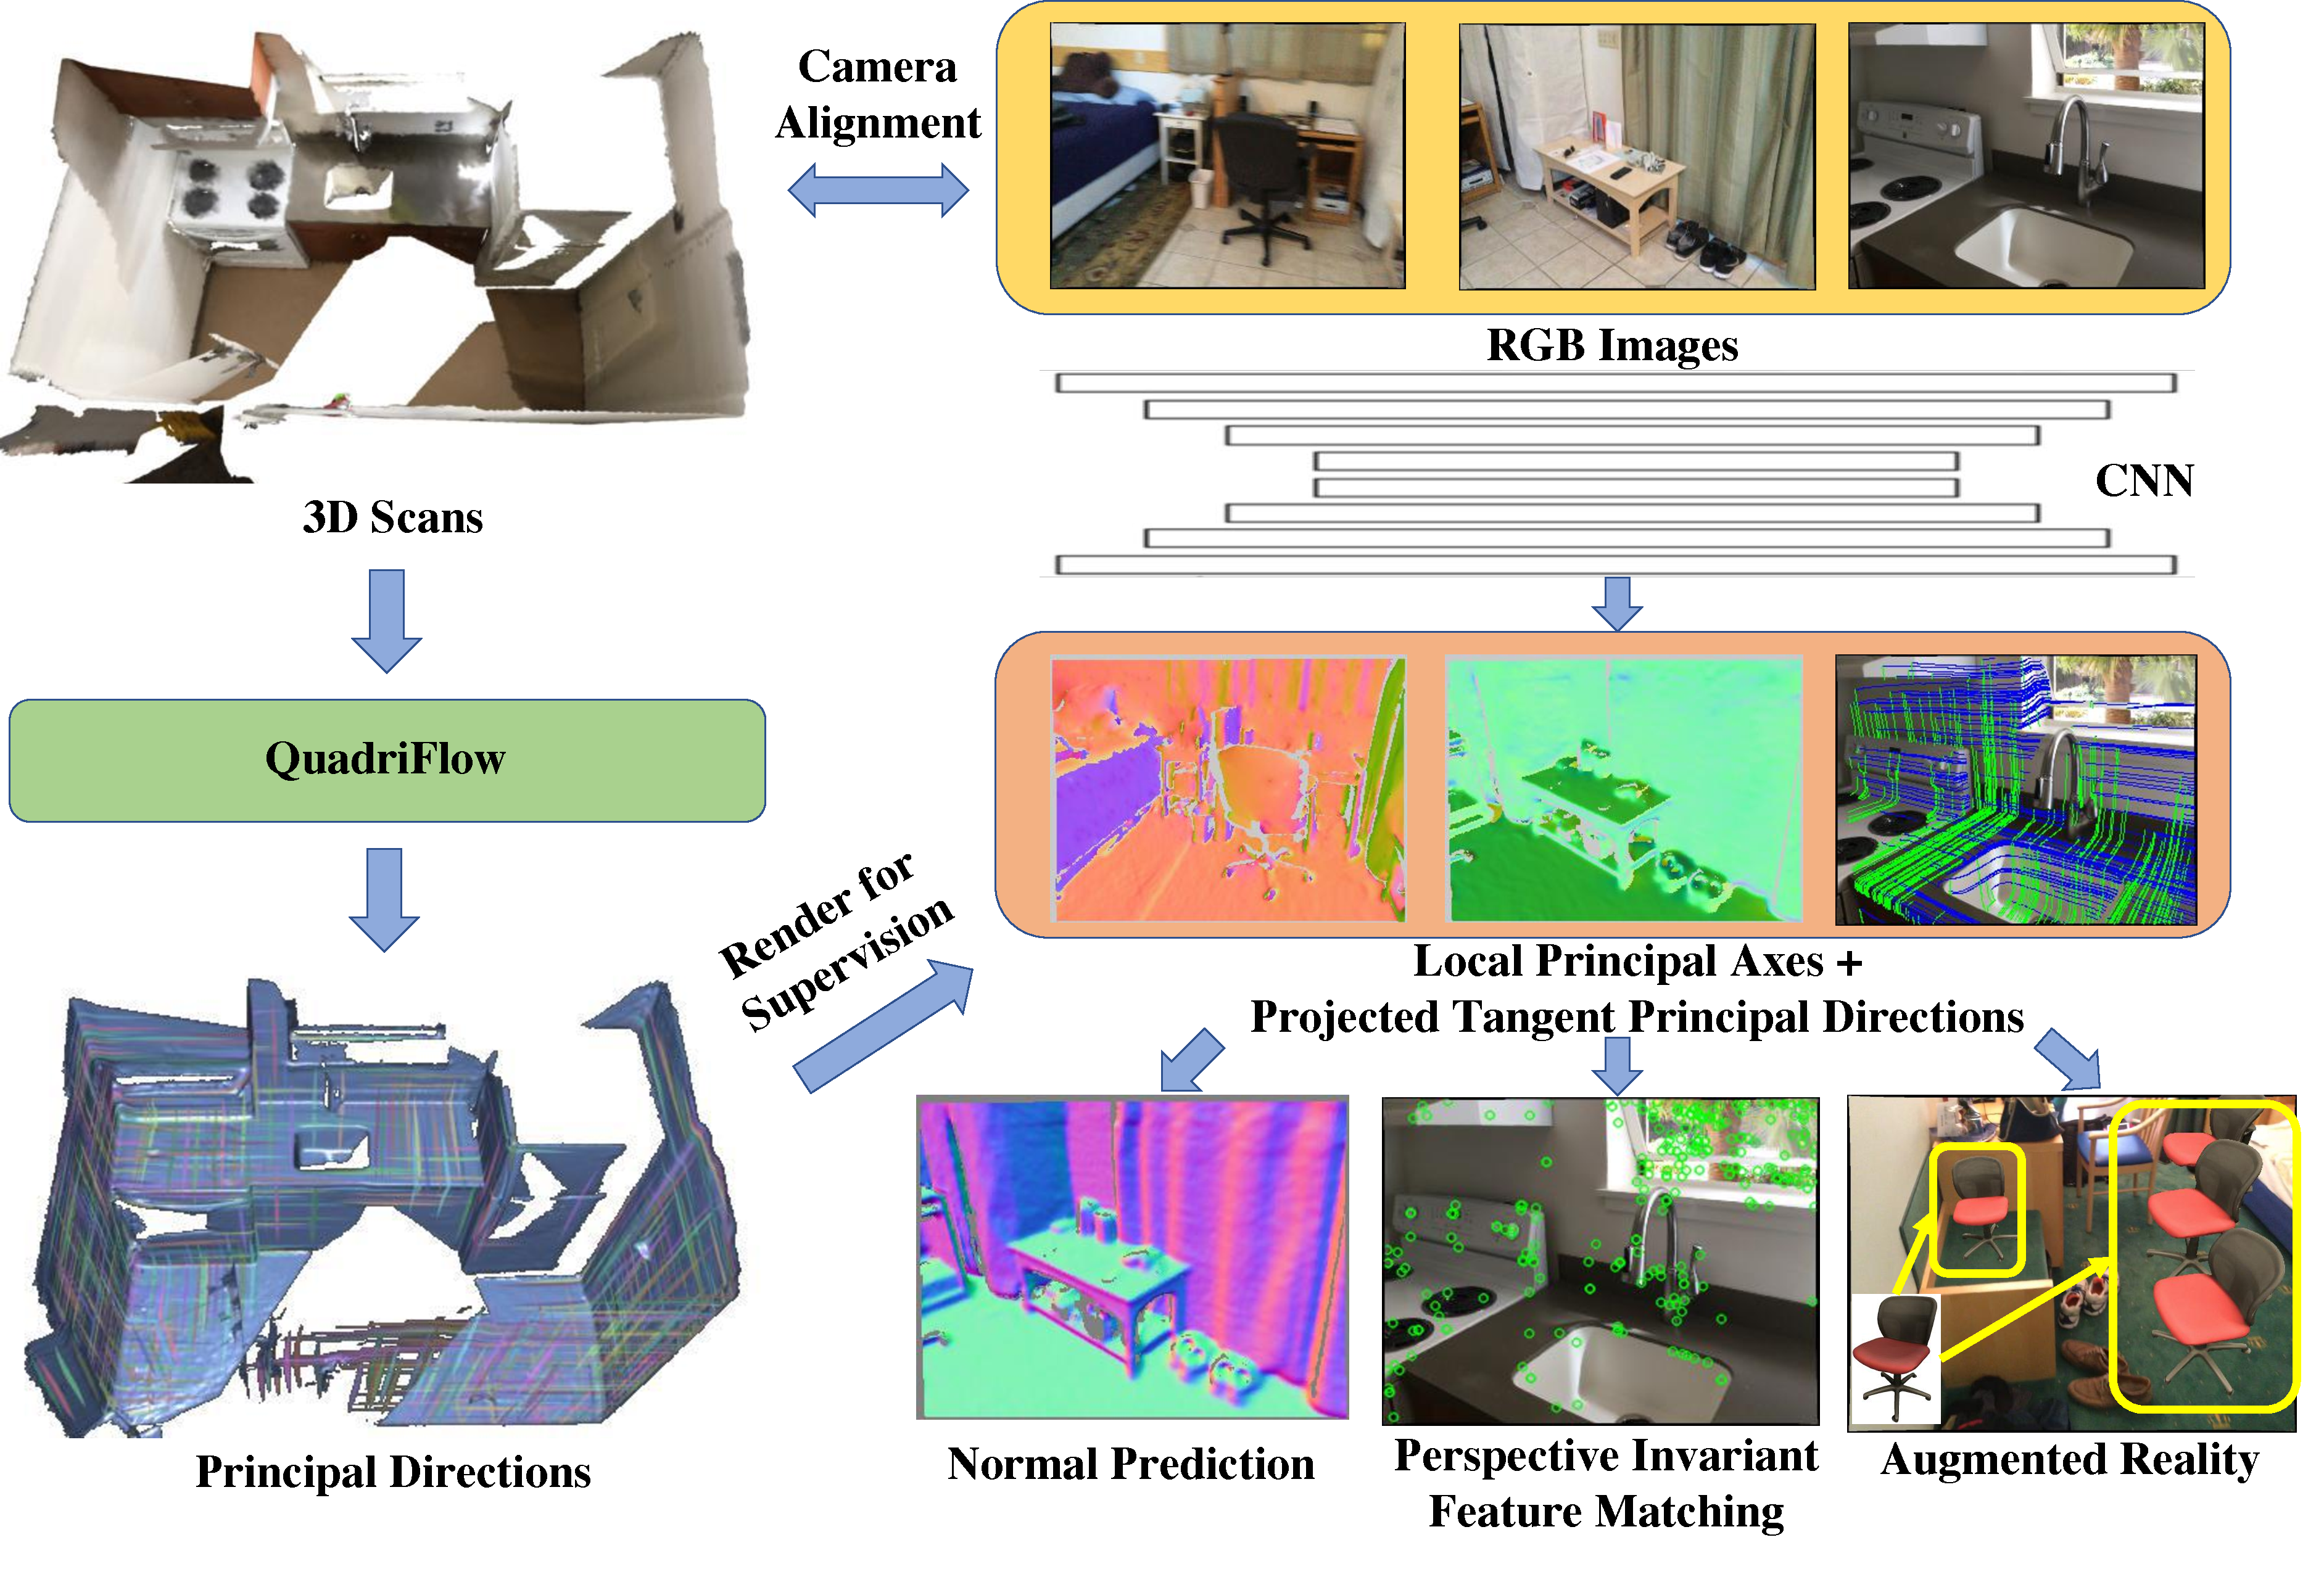
\includegraphics[width=0.75\linewidth]{FrameNet/graph/teaser.pdf}
    \caption{We propose the novel task of predicting dense 3D \cframe{} from a single RGB image. We compute the frames from reconstructed meshes using QuadriFlow and render them to images to supervise the task.  We train a network that predicts all directions of the frames jointly.  We find that predicted tangents provides better surface normals, and are useful for applications like feature matching and augmented reality.}
    \label{fig:framenet-teaser}
    \vspace{-0.1in}
\end{figure}
The seamless surface parameterization is itself an important feature that is strongly correlated with the RGB signals. The edge orientations of our quad mesh are aligned with the tangent principal directions. At the same time, we observe that each pixel in an image is the projection of a small surface region in the underlying 3D geometry, where a canonical frame can be identified as represented by three orthogonal axes, one along its normal direction and two along tangent principal directions specified by the quad edges. Therefore, we introduce FrameNet~\cite{framenet} as a novel image-to-3D task: dense 3D \cframe{} estimation from a single image (figure~\ref{fig:framenet-teaser}).

In fact, the image-to-3D tasks have made great progress in recent years.  For example, monocular depth estimation~\cite{shelhamer2015scene,li2017two,xu2017multi,wang2018adaptive,fu2018deep} and surface normal prediction~\cite{eigen2015predicting,wang2015designing,bansal2016marr,qi2018geonet} have improved dramatically.  There are many applications for these tasks in scene understanding and robot interaction.
%
The main challenge in this domain is choosing an appropriate representation of 3D geometry to predict.  Zhang~\textit{et al.}~\cite{zhang2018deep} predict dense surface normals and then use geometric constraints to solve for depth with global optimization.  GeoNet~\cite{qi2018geonet} predicts both surface normals and depth and then passes them to a refinement network for further optimization.  These methods are clever in their use of geometric constraints to regularize dense predictions.   However, they infer only 2 of the 3 degrees of freedom in a 3D coordinate frame -- the rotation in the tangent plane around the surface normal is left unknown.  As such, they are missing 3D information critical to many applications.   For example, they cannot assist an AR system in placing a picture frame on a wall or a laptop on a table because they don't know the full 3D coordinate frame (including tangent directions) of the wall or table surfaces.

Our task instead requires predicting a full 3D coordinate frame defined by the surface normal {\em and two principal tangent directions} of the surface observed at every pixel in an RGB image.  We investigate this task for three reasons.   First, we expect that predicting principal tangent directions is easier than predicting normals because they are often aligned with observable patterns in surface textures (e.g., wood grains, fabric weaves, tile seams, etc.) and surface boundaries, which are directly observable in images.  Second, we expect that joint surface normal and tangent prediction is more robust than normal prediction alone due to the regularization provided by orthogonality constraints.  Third, we expect that predicting a full canonical 3D coordinate frame at every pixel is useful for many applications, such as augmented reality.

\cam{We have implemented an algorithm for this task in a supervised setting.   To acquire ``ground truth'' \cframe{}, we leverage data from RGB-D scanning datasets, like ScanNet~\cite{dai2017scannet}, which provide large sets of images posed within reconstructed 3D meshes.  
We compute \cframe{} on the meshes and render them to the RGB images to produce training data.  There are multiple choices for how to define the frames.  A simple approach would be to use Manhattan frames; however, they
reflect only the global scene orientation %(figure~\ref{fig:framenet-vis-direction}(a))
.   Instead, we compute locally consistent 4-RoSy \cframe{} that follow principal curvatures using the Quadriflow algorithm~\cite{huang2018quadriflow} %(figure~\ref{fig:framenet-vis-direction}(b))
.  We find that the surface tangent directions computed this way are consistent with image features and can be learned by a network from 2D data.}

\cam{The \cframes{} are fundamental 3D properties of a scene, as they imply the canonical transformation that maps the 3D surface to the image plane.  They provide not only the surface normal but also canonical tangent directions and their projections onto the image plane.  We show that predicting all these directions jointly can improve surface normal estimation, local patch description using SIFT features~\cite{lowe2004distinctive}, and allow the insertion of novel objects with correct orientation in augmented reality applications.}

\section{Contributions and Thesis Outlines}
\label{intro:contribution}
\begin{figure}
    \centering
    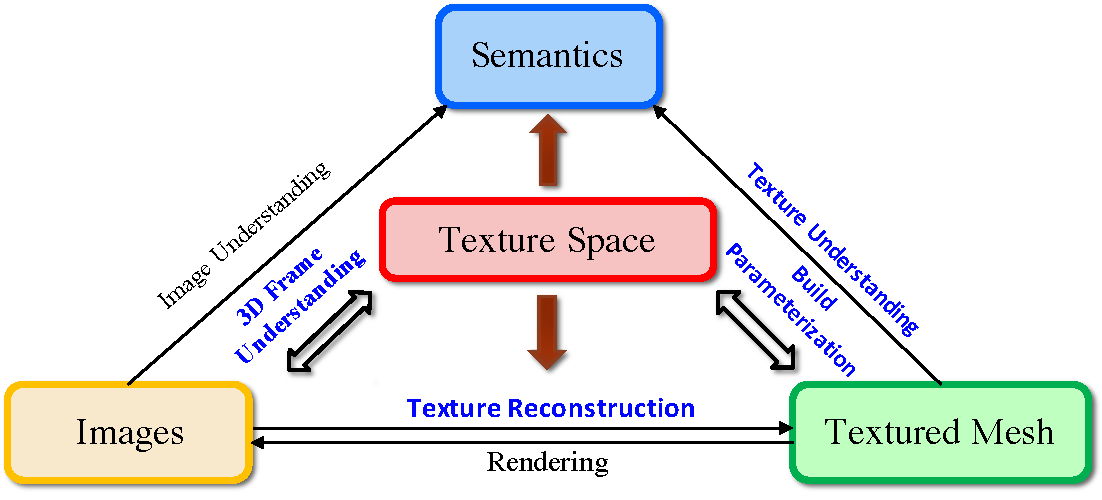
\includegraphics[width=0.75\linewidth]{intro/concept.pdf}
    \caption{Our works focus on surface texture processing to reconstruct and understand the environment. Our problems are marked using blue fonts. We reconstruct the surface texture based on images from the scans, build a seamless parameterization to create a texture space, and propose a texture convolution operator in such a space to understand the semantics. We further explore the understanding of the parameterization from the images.}
    \label{fig:intro-concept}
\end{figure}
This thesis mainly focuses on surface texture processing. In summary, figure~\ref{fig:intro-concept} illustrates the main components related to the surface texture. where our problems are marked using blue fonts. Basically, the surface texture has a strong relationship with the scanning images via rendering and reconstruction. We focus on reconstructing high-quality surface textures from images. We propose to construct the texture space using the seamless surface parameterization. This leads to an important representation that is helpful for texture understanding including the semantics understanding from parameterized textures and canonical frame understanding from images.

We discuss the related works in chapter~\ref{chapter:related}. Texture optimization is based on color consistency optimization~\cite{huang20173dlite} or joint adversarial metric optimization~\cite{huang2020adversarial}, as described in chapter~\ref{chapter:texture-recon}. For understanding, we first solve the fundamental surface parameterization problem~\cite{huang2018quadriflow} as explained in chapter~\ref{chapter:param}, and design a network with 2D convolution operators~\cite{huang2018texturenet} under the canonical surface parameterization (chapter~\ref{sec:texturenet}. Observing the correlation between surface parameterization and texture signals, we propose to learn canonical frames from RGB images~\cite{framenet} in chapter~\ref{sec:framenet}. Finally, we draw the conclusions and discuss about the future directions for surface texture processing in chapter~\ref{chapter:conclude}.

Overall, the contributions of this thesis include:
\begin{itemize}
    \item Identify the surface processing problem as to reconstruct the texture, parameterize the texture space and understand the texture.
    \item We propose \emph{3DLite} as an approach to produce high-quality surface textures on top of the lightweight planar geometry abstracted from the scan.
    \item We propose an \emph{adversarial texture optimization} method to produce photorealistic textures for approximate surfaces, even from misaligned images, by learning an objective function that is robust to scanning errors.
    \item We propose \emph{Quadriflow} as a scalable and robust quadrangulation algorithm that is solvable in polynomial time.
    \item Based on consistent local parameterizations from \emph{Quadriflow}, we design \emph{TextureNet} as a novel neural network for extracting features from high-resolution signals living on surfaces embedded in 3D.
    \item We observe the high correlation between surface parameterization from \emph{Quadriflow} and RGB signals on surface texture, and identify an important new 3D vision problem with a solution called \emph{FrameNet}: local canonical frame estimation from RGB images.
\end{itemize}
